\documentclass{exam}

\usepackage{siunitx} 
\usepackage{graphicx}
\usepackage[fleqn]{amsmath}
\usepackage{cancel}
\usepackage{float}
\usepackage{mdwlist}
\usepackage{booktabs}
\usepackage{cancel}
\usepackage{polynom}
\usepackage{caption}
\usepackage{fullpage}
\usepackage{comment}

\newcommand{\degree}{\ensuremath{^\circ}} 
\everymath{\displaystyle}

% \begin{figure}[H]
%   \centering
%   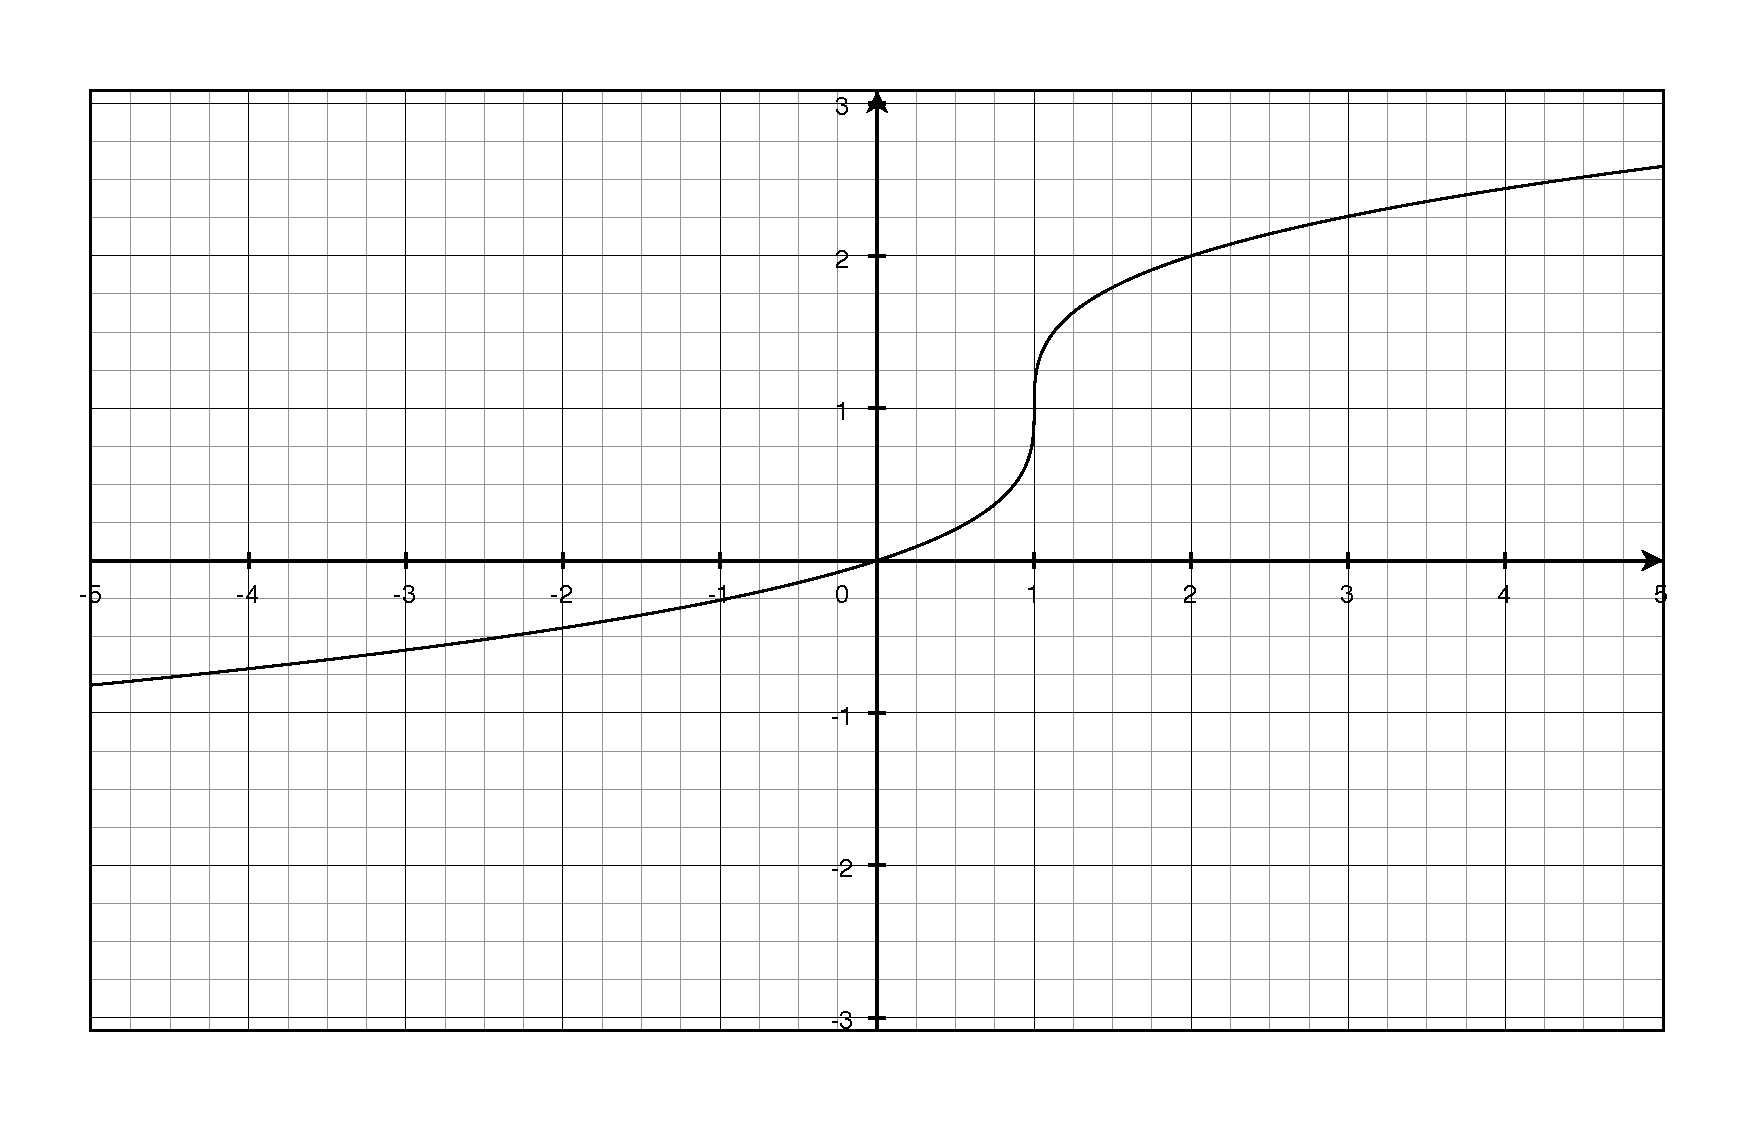
\includegraphics[scale=.3]{question7.eps}
%   \caption*{question 7}
% \end{figure}

% \begin{tabular}{cc}
% \toprule
% period & amplitude \\
% \midrule
%   $\pi$ & $2$ \\
% \bottomrule
% \end{tabular}

\printanswers
\excludecomment{comment}

\ifprintanswers 
  \usepackage{2in1, lscape} 
\fi

\author{}
\date{January 9, 2013}
\title{Math 141 \\ Homework One}

\begin{document}

\maketitle

\section{Homework}

\begin{itemize*}
  \item Skim Chapter 1.  This chapter should mostly be review from the algebra class.
  \item Read section 2.1
  \item Section 2.1: 1-8, 11-12, 15-16, 19-22, 24-30, 33, 41-45, 55-59, 61, 65
\end{itemize*}

\section{Extra Credit}

Page 143, problem 20.

\ifprintanswers
  \begin{solution}
    If you draw a cross section of the pyramid and label the height of the part that has been chopped off as $h_t$, you
    can see that there are similar triangles.  This lets us come up with the following equation:
    \[
      \frac{b/2}{h_t} = \frac{a/2}{h + h_t}
    \]
    Solve for $h_t$:
    \[
      h_t = h \cdot \left( \frac{b}{a - b} \right)
    \]

    The volume of the truncated pyramid is the volume of the whole pyramid minus the volume of the part that has been
    chopped off:
    \begin{align*}
      V &= \frac{1}{3} a^2 \left(h + \frac{bh}{a - b} \right) - \frac{1}{3} b^2 \left( \frac{bh}{a - b} \right) \\
      &= \frac{1}{3} h \left( \frac{a^3 - b^3}{a - b} \right) \\
    \end{align*}

    This doesn't look like the desired answer.  But if you remember the formula for factoring the difference of two cubes,
    you can factor the numerator.  Even if you don't remember the formula, you can look at the goal, and verify that
    $a^3 - b^3 = (a - b)(a^2 + ab + b^2)$.  So the preceding equation simplifies to:
    \begin{align*}
      \frac{1}{3} h \left( \frac{a^3 - b^3}{a - b} \right) 
        &= \frac{1}{3} h \left( \frac{\cancel{(a - b)}(a^2 + ab + b^2)}{\cancel{a - b}} \right) \\
        &= \frac{1}{3} h (a^2 + ab + b^2) \\
    \end{align*}
  \end{solution}

  % Imagine that you have three boxes. One contains two black marbles, one contains two white marbles, and the third,
  % one black marble and one white marble. The boxes were labeled for their contents---BB, BW, WW---but someone switched the
  % labels so that every box is now incorrectly labeled. You are allowed to take one marble at a time out of any box,
  % without looking inside, and by this process of sampling you are to determine the contents of all three boxes. What is
  % the smallest number of drawings needed to do this?
  % 
  % \begin{solution}
  %   You can identify all the boxes by taking a single marble from the BW box.  You know all the boxes are labeled
  %   incorrectly, so this box is actually either the WW box or the BB box.  You can tell which of these it is by the color
  %   of the marble.
  % 
  %   Suppose you draw a white marble.  You now know that the box labeled BW is actually the WW box.  You have two boxes
  %   left to identify, and you know that they are both labeled incorrectly.  Therefore, the box labeled WW must be the BB
  %   box and the box labeled BB must be the BW box.
  % 
  %   Similar reasoning applies if the marble you draw originally is black.
  % \end{solution}

  \pagebreak

  \section{Section 2.1}
  \begin{description}
    \item[1]
      \[
        f(x) = 2(x + 3)
      \]

    \item[2]
      \[
        f(x) = \frac{x}{7} - 4
      \]

    \item[3]
      \[
        f(x) = (x - 5)^2
      \]

    \item[4]
      \[
        f(x) = \frac{1}{3} (\sqrt{x} + 8)
      \]

    \item[5] subtract 4, then divide by 3.

    \item[6] divide by 3, then subtract 4.

    \item[7] square, then add 2.

    \item[8] add 2, then take square root.

    \item[11]
      \[
        f(x) = 2(x - 1)^2
      \]
      \begin{tabular}{lrrrrr}
        \toprule
        $x$    & $-1$ & $0$ & $1$ & $2$ & $3$ \\
        $f(x)$ & $8$  & $2$ & $0$ & $2$ & $8$ \\
        \bottomrule
      \end{tabular}

    \item[12]
      \[
        g(x) = | 2x + 3 |
      \]
      \begin{tabular}{lrrrrr}
        \toprule
        $x$    & $-3$ & $-2$ & $0$ & $1$ & $3$ \\ 
        $f(x)$ &  $3$ &  $1$ & $3$ & $5$ & $9$ \\ 
        \bottomrule
      \end{tabular}

    \item[15]
      \[
        g(x) = \frac{1 - x}{1 + x}
      \]

      \begin{tabular}{lrrrrrr}
        \toprule
        $x$      & $2$    & $-2$ & $1/2$ & $a$                   & $a - 1$           & $-1$ \\
        \midrule
        $f(x)$   & $-1/3$ & $-3$ & $1/3$ & $\frac{1 - a}{1 + a}$ & $\frac{2 - a}{a}$ & undefined \\
        \bottomrule
      \end{tabular}

\begin{comment}
  *****
    write ``undefined'' instead of $x \neq -1$.
  *****
\end{comment}

    \item[16]
      \[
        h(t) = t + \frac{1}{t}
      \]

      \begin{tabular}{lrrrrrr}
        \toprule
        $t$    & $1$ & $-1$ &   $2$ & $5/2$ &       $x$ &     $1/x$ \\ 
        \midrule
        $f(t)$ & $2$ &  $-2$ & $5/2$ & $5/2$ & $x + 1/x$ & $x + 1/x$ \\ 
        \bottomrule
      \end{tabular}

    \item[19]
      \[
        f(x) = 2 |x - 1|
      \]

      \begin{tabular}{lrrrrrr}
        \toprule
        $x$    & $-2$ & $0$ & $1/2$ & $2$ & $x + 1$ & $x^2 + 2$ \\ 
        \midrule
        $f(x)$ & $6$ &  $2$ &   $1$ & $2$ & $2 |x|$ & $2 |x^2 + 1|$ \\ 
        \bottomrule
      \end{tabular}

\begin{comment}
  *****
  You can't get rid of the absolute value sign in the $|x|$ case because $x$ might be negative.  It is OK to remove it
  for the $x^2 + 1$ case, since $x^2 + 1$ is always positive.
  *****
\end{comment}

    \item[20]
      \[
        f(x) = \frac{|x|}{x}
      \]

      \begin{tabular}{lrrrrrr}
        \toprule
        $x$      & $-2$ & $-1$ & $0$       & $5$ & $x^2$ & $1/x$ \\
        \midrule
        $f(x)$   & $-1$ & $-1$ & undefined & $1$ & $1$   & $|x|/x$ \\
        \bottomrule
      \end{tabular}

      $\frac{|x|}{x} = -1$ when $x < 0$, so you can't simplify this case to $1$.  Since $x^2$ is always greater than or
      equal to zero, it is OK to simplify $\frac{|x^2|}{x^2}$ to 1.

\begin{comment}
  *****
  $\frac{0}{0} \neq 1$
  *****
\end{comment}

\pagebreak

    \item[21]
      \[
        f(x) = 
          \begin{cases}
            x^2   & \text{if } x < 0 \\
            x + 1 & \text{if } x \geq 0 \\
          \end{cases}
      \]

      \begin{tabular}{lrrrrr}
        \toprule
        $x$      & $-2$ & $-1$ & $0$ & $1$ & $2$ \\
        \midrule
        $f(x)$   & $4$  & $1$  & $1$ & $2$ & $3$ \\
        \bottomrule
      \end{tabular}

    \item[22]
      \[
        f(x) = 
          \begin{cases}
            5      & \text{if } x \leq 2 \\
            2x - 3 & \text{if } x > 2 \\
          \end{cases}
      \]

      \begin{tabular}{lrrrrr}
        \toprule
        $x$    & $-3$ & $0$ & $2$ & $3$ & $5$ \\ 
        \midrule
        $f(x)$ &  $5$ & $5$ & $5$ & $3$ & $7$ \\
        \bottomrule
      \end{tabular}

    \item[24]
      \[
        f(x) = 
          \begin{cases}
            3x        & \text{if } x < 0 \\
            x + 1     & \text{if } 0 \leq x \leq 2 \\
            (x - 2)^2 & \text{if } x > 2 \\
          \end{cases}
      \]

      \begin{tabular}{lrrrrr}
        \toprule
        $x$    &  $-5$ & $0$ & $1$ & $2$ & $5$ \\ 
        \midrule
        $f(x)$ & $-15$ & $1$ & $2$ & $3$ & $9$ \\
        \bottomrule
      \end{tabular}
      
      \item[25]
      \begin{align*}
        f(x + 2)     &= (x + 2)^2 + 1 \\
                     &= x^2 + 4x + 5 \\
        f(x) + f(2)  &= (x^2 + 1) + (2^2 + 1) \\
                     &= x^2 + 6 \\
      \end{align*}

    \item[26]
      \begin{align*}
        f(2x)  &= 3 \cdot 2x - 1 \\
               &= 6x - 1 \\
        2 f(x) &= 2 (3x - 1) \\
               &= 6x - 2 \\
      \end{align*}

      \item[27]
      \begin{align*}
        f(x^2)   &= x^2 + 4 \\
        (f(x))^2 &= (x + 4)^2 \\
                 &= x^2 + 8x + 16 \\
      \end{align*}

    \item[28]
      \begin{align*}
        f(x)                         &= 6x - 18 \\
        f \left( \frac{x}{3} \right) &= 6 \cdot \frac{x}{3} - 18 \\
                                     &= 2x - 18 \\
        \frac{f(x)}{3}               &= \frac{6x - 18}{3} \\
                                     &= 2x - 6 \\
      \end{align*}

    \item[29]
      \[
        f(x) = 3x + 2
      \]
      \begin{align*}
        f(a)     &= 3a + 2 \\
        f(a + h) &= 3(a + h) + 2 \\
        \\
        q        &= \frac{3(a + h) + 2 - (3a + 2)}{h} \\
                 &= \frac{3a + 3h + 2 - 3a - 2}{h} \\
                 &= \frac{3h}{h} \\
                 &= 3 \\
      \end{align*}

    \pagebreak

    \item[30]
      \[
        f(x) = x^2 + 1
      \]
      \begin{align*}
        f(a)     &= a^2 + 1 \\
        f(a + h) &= (a + h)^2 + 1 \\
        \\
        q &= \frac{(a + h)^2 + 1 - (a^2 + 1)}{h} \\
          &= \frac{a^2 + 2ah + h^2 + 1 - a^2 - 1}{h} \\
          &= \frac{2ah + h^2}{h} \\
          &= 2a + h \\
      \end{align*}

    \item[33]
      \[
        f(x) = \frac{x}{x + 1}
      \]
      \begin{align*}
        f(a)     &= \frac{a}{a + 1} \\
        f(a + h) &= \frac{a + h}{a + h + 1} \\
        \\
        q        &= \frac{\left( \cfrac{a + h}{a + h + 1} - \cfrac{a}{a + 1} \right) }{h} \\
                 &= \frac{\left( \cfrac{a^2 + a + ah + h - (a^2 + ah + a)}{(a + h + 1)(a + 1)} \right)}{h} \\
                 &= \frac{a^2 + a + ah + h - a^2 - ah - a}{h(a + h + 1)(a + 1)} \\
                 &= \frac{1}{(a + h + 1)(a + 1)} \\
      \end{align*}

    \item[41] The denominator is 0 when $x = 3$, so the range is $x \neq 3$.

    \item[42] The denominator is 0 when $x = 2$, so the range is $x \neq 2$.  

    \item[43] The denominator is 0 when $x = \pm 1$, so the range is $x \neq \pm 1$.

    \item[44]
      The denominator is 0 when 
      \begin{align*}
        x^2 + x - 6    &= 0 \\
        (x + 3)(x - 2) &= 0 \\
        x              &= \left\{ -3, 2 \right\} \\
      \end{align*}

      So the range is $x \neq \left\{ -3, 2 \right\}$.

    \item[45]
      The function is defined when the value inside the square root is not negative, so the range is $[5, \infty)$.

    \item[55]
      \begin{align*}
        x - 4 &> 0 \\
        x     &> 4 \\
      \end{align*}

    \item[56]
      \begin{align*}
        6 - x &> 0 \\
        x     &< 6 \\
      \end{align*}

    \item[57]
      \begin{align*}
        2x - 1 &> 0 \\
        x      &> \frac{1}{2} \\
      \end{align*}

    \item[58]
      \begin{align*}
        9 - x^2 &> 0 \\
        x^2     &< 9 \\
      \end{align*}
      \[
        -3 < x < 3
      \]

    \item[59]
      \begin{parts}
        \part
          \begin{align*}
            C(10)  &= \$1,532.10 \\
            C(100) &= \$2,100.00 \\
          \end{align*}

          \part These are the costs to make 10 and 100 yards.

          \part $C(0) = \$1,500$, which is the cost of keeping the factory open, paying the rent, etc., without actually
          making anything.
      \end{parts}

    \item[61]
      \begin{parts}
        \part
          \begin{align*}
            D(0.1) &\approx \SI{28.1}{mile} \\
            D(0.2) &\approx \SI{39.8}{mile} \\
          \end{align*}

          \part $\SI{1135}{ft} = \frac{1135}{5280} \approx \SI{0.215}{mi}$

          $D(0.215) \approx \SI{41.3}{mile}$

          \part $D(7) \approx \SI{253.6}{mile}$
      \end{parts}

    \item[65]
      \begin{parts}
        \part
          \begin{align*}
            L(0.5c)  &\approx \SI{8.66}{m} \\
            L(0.75c) &\approx \SI{6.61}{m} \\
            L(0.9c)  &\approx \SI{4.36}{m} \\
          \end{align*}

          \part It appears to be shorter. 
      \end{parts}
      
  \end{description}
\else
  \vspace{10 cm}

  I claim credit for nothing. Everything is determined, the beginning as well as the end, by forces over which we have no
  control. It is determined for the insect as well as for the star. Human beings, vegetables or cosmic dust, we all dance
  to a mysterious tune, intoned in the distance by an invisible player. 

  \vspace{.2 cm}

  \hspace{1 cm} --Albert Einstein

\fi

\end{document}

